\documentclass[11pt]{article}

\usepackage[margin=1.1in]{geometry}
\usepackage{amsmath,amssymb,amsthm}
\usepackage{mathtools}
\usepackage{booktabs}
\usepackage{tikz}
\usetikzlibrary{arrows.meta,positioning,fit,backgrounds}
\usepackage{xcolor}
\usepackage{enumitem}
\usepackage[colorlinks=true,linkcolor=blue!60!black,citecolor=blue!60!black,urlcolor=blue!60!black]{hyperref}
\usepackage{microtype}
\usepackage{graphicx}

\newtheorem{theorem}{Theorem}[section]
\newtheorem{lemma}[theorem]{Lemma}
\newtheorem{definition}[theorem]{Definition}
\newtheorem{example}[theorem]{Example}
\newtheorem{claim}[theorem]{Claim}
\newtheorem{openq}[theorem]{Open Question}
\newtheorem*{finding}{Finding}

% Paper-style notation (shared with joinpeel-note.tex)
\newcommand{\vis}{\xrightarrow{\mathsf{vis}}}
\newcommand{\rc}{\xrightarrow{\mathsf{rc}}}
\newcommand{\loC}{\xrightarrow{\mathsf{lo}_{C}}}
\newcommand{\comm}{\rightleftarrows}
\newcommand{\ncomm}{\not\rightleftarrows}
\newcommand{\add}{\mathsf{add}}
\newcommand{\rem}{\mathsf{rem}}
\newcommand{\enb}{\mathsf{enable}}
\newcommand{\dsb}{\mathsf{disable}}
\newcommand{\Merge}{\mathsf{merge}}
\newcommand{\mergeL}{\mathsf{mergeL}}
\newcommand{\Sinit}{\sigma_0}
\newcommand{\loE}[1]{\mathsf{lo}^{#1}}
\newcommand{\dow}[1]{{\downarrow}#1}
\newcommand{\co}{\mathsf{CoreVCs3CD}}
\newcommand{\fd}{\mathsf{FeasibleDeltaVCs3}}
\newcommand{\cd}{\mathsf{CDVC3}}
\newcommand{\lean}[1]{\texttt{#1}}

\title{\bfseries Eight Verification Conditions for MRDTs:\\
\large a mechanized, corrected soundness metatheory for RA-linearizability
under three-way merge, with nine production data types discharged}
\author{Sal metatheory note\\ \small FP Launchpad, IIT Madras}
\date{July 3, 2026}

\begin{document}
\maketitle

\begin{abstract}
\noindent
Mergeable replicated data types (MRDTs) resolve concurrent divergence by a
\emph{three-way} merge $\mergeL(l,a,b)$: the two divergent states $a,b$
are reconciled relative to their lowest common ancestor $l$ in a git-like
version DAG. The Neem methodology reduces RA-linearizability of an MRDT to
a fixed catalogue of per-data-type verification conditions (VCs), tied
together by a once-and-for-all soundness meta-theorem. A companion
note\footnote{\emph{Set-relative linearization and the Join Lemma}
(\texttt{joinpeel-note.pdf}, same directory), which treats the binary
(CRDT) specialization and develops the corrected proof architecture reused
here.} shows that the meta-theorem's proof is unsound as written and that
its VC catalogue is insufficient; this note lifts the corrected
architecture to the \emph{ternary} setting the paper actually claims. The
lift is not routine: the LCA argument is load-bearing (the counter MRDT is
provably outside the binary theorem), the paper's own LCA lemma has a gap
in its proof, and the lattice-flavoured repair that works for CRDTs
provably does not survive (no idempotence, no usable order). What survives
is a \emph{delta} discipline: three unconditional relational VCs on
$\mathsf{rc}$, one merge symmetry, three \emph{feasibility-conditioned}
redistribution laws, and a single contextual \emph{causal-delta} equation
--- eight VCs in all --- from which every reachable configuration of the
replicated store is RA-linearizable, \emph{per version}. All of it is
mechanized in Lean~4 with zero \lean{sorry}s, and the VC set is validated
in the strongest currency available: nine of the twelve production MRDTs
of the Sal repository --- including OR-sets, an enable-wins flag,
counters, a tombstone RGA and Peritext --- carry kernel-checked
end-to-end RA-linearizability theorems through it.
\end{abstract}

\tableofcontents

\section{Introduction}

An MRDT execution looks like a git history: replicas fork, apply
operations locally, and merge. Unlike a state-based CRDT, whose binary
merge must reconcile two states with no memory of their common past, an
MRDT's merge receives a third argument --- the state at the \emph{lowest
common ancestor} (LCA) of the two versions being merged --- and may use it
to compute \emph{deltas}: what each side did since the fork. The
paradigmatic example is the counter,
\[
  \mergeL(l,a,b) \;=\; a + b - l,
\]
which adds the two sides' increments-since-$l$ instead of double-counting
their common past (Figure~\ref{fig:counter}).

\begin{figure}[t]
\centering
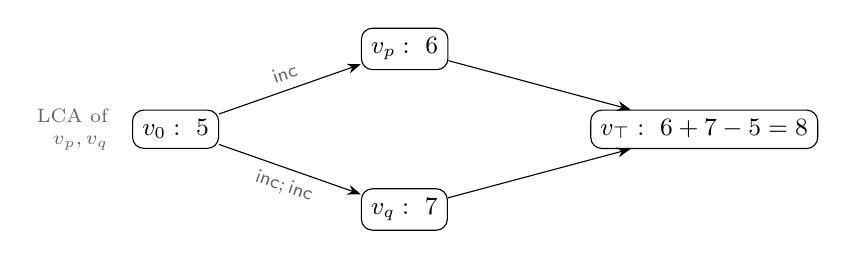
\begin{tikzpicture}[>=Stealth, node distance=0.75cm and 1.5cm,
  ver/.style={draw, rounded corners, inner sep=3.5pt, font=\small},
  lbl/.style={font=\scriptsize, text=black!60}]
\node[ver] (v0) {$v_0:\ 5$};
\node[ver, above right=0.5cm and 1.8cm of v0] (a1) {$v_p:\ 6$};
\node[ver, below right=0.5cm and 1.8cm of v0] (b1) {$v_q:\ 7$};
\node[ver, below right=0.5cm and 1.8cm of a1] (m) {$v_\top:\ 6+7-5 = 8$};
\draw[->] (v0) -- node[lbl, above, sloped]{$\mathsf{inc}$} (a1);
\draw[->] (v0) -- node[lbl, below, sloped]{$\mathsf{inc};\mathsf{inc}$} (b1);
\draw[->] (a1) -- (m);
\draw[->] (b1) -- (m);
\node[lbl, left=0.18cm of v0, align=right] {LCA of\\$v_p,v_q$};
\end{tikzpicture}
\caption{The counter MRDT. Both branches inherit the $5$ from the fork
point; the LCA argument lets the merge count each branch's \emph{delta}
exactly once. No binary merge of $6$ and $7$ alone can recover $8$: the
information ``how much is shared'' lives in the DAG, and the LCA argument
is how the data type reads it.}
\label{fig:counter}
\end{figure}

The Neem methodology (OOPSLA~2025) promises a clean division of labour:
the data-type designer discharges a fixed catalogue of equations over
$\mathsf{do}$, $\mergeL$ and the conflict-resolution relation
$\mathsf{rc}$ --- mostly by SMT --- and a soundness meta-theorem, proved
once, converts those VCs into \emph{RA-linearizability} of every reachable
configuration. The companion note documents what a Lean~4 mechanization
found in the binary specialization: the meta-theorem's central induction
is unsound as written, and the VC catalogue is insufficient --- there are
reachable, VC-satisfying executions that are not RA-linearizable. It also
develops the repair: a set-relative linearization order, canonical states
$\sigma(E)$, and a \emph{Join Lemma} whose induction consumes a small,
contextual VC surface.

This note is about the setting the paper actually claims: \textbf{ternary
merge over a version DAG}. Its contributions:

\begin{enumerate}[leftmargin=2em]
\item \textbf{The ternary lift is not an inert third argument}
  (\S\ref{sec:loadbearing}): the counter satisfies the ternary shared-peel
  VC but \emph{provably violates} its binary counterpart, so the class of
  MRDTs covered by the ternary theorem strictly exceeds anything the
  binary theorem can reach. ``A CRDT is an MRDT that ignores its LCA'' is
  a one-way instantiation, not an equivalence.
\item \textbf{The paper's LCA lemma is true but its proof has a gap}
  (\S\ref{sec:lca}): $L(v_\top) = L(v_1) \cap L(v_2)$ holds, but only as a
  \emph{reachability invariant} of the store, whose proof needs a
  generator-uniqueness induction the paper silently assumes. We mechanize
  the transition system and the invariant. The binary defeater
  configuration also lifts, verbatim, to a fully LCA-legal ternary
  execution (\S\ref{sec:defeater}).
\item \textbf{The lattice repair provably does not survive the lift}
  (\S\ref{sec:whydelta}): MRDT merges are not idempotent
  ($\mergeL(l,a,a)=2a-l$ for the counter), the induced orders degenerate,
  and the honest associativity law has \emph{four distinct LCAs} and holds
  only on feasible tuples. What replaces the lattice laws is a two-law
  \emph{delta contract} --- redistribution identities in which the LCA
  slot does, by arithmetic, the job idempotence did order-theoretically.
\item \textbf{Eight VCs suffice} (\S\ref{sec:vcs}--\S\ref{sec:adequacy}):
  three relational VCs on $\mathsf{rc}$ (one of them carrying a
  different-replica guard that restores the paper's own F\textsuperscript{*}
  artifact interface --- the Lean transcription had dropped it, and a real
  data type detects the drop), merge symmetry, three
  feasibility-conditioned delta laws, and one contextual \emph{causal-delta}
  equation. The adequacy theorem is per \emph{version}: every version in
  the store, LCAs included, linearizes.
\item \textbf{The VC set is validated on the production catalogue}
  (\S\ref{sec:catalog}): nine of the twelve MRDTs shipped in Sal ---
  OR-set, an optimized OR-set, enable-wins flag, grow-only set and map,
  increment-only and PN counters, a tombstone RGA, and Peritext --- are
  discharged end-to-end, kernel-checked. The sweep produces an empirical
  \emph{class map} of which data types need which strength of contract,
  with two surprises: tombstones are a metatheoretic trivializer, and
  commutativity class and delta class are independent axes.
\end{enumerate}

Everything stated as a theorem below is mechanized with zero
\lean{sorry}s; \S\ref{sec:mech} maps statements to Lean names and files.

\section{The ternary setting}
\label{sec:setting}

\paragraph{Signature.} An MRDT is $\langle \Sigma, \Sinit, \mathsf{do},
\mergeL, \mathsf{rc}\rangle$: a state space with initial state, an update
function applied to \emph{events} $e = (t, r, o)$ (a globally fresh
timestamp, an origin replica, an operation), a ternary merge, and a
conflict-resolution relation $\mathsf{rc}$ on operations used to order
concurrent non-commuting pairs. We write $e(\sigma)$ for
$\mathsf{do}(\sigma,e)$, and $e_1 \comm e_2$ when
$e_1(e_2(\sigma)) = e_2(e_1(\sigma))$ for every $\sigma$.

\paragraph{Executions.} A configuration carries a \emph{store}: a DAG of
versions, each holding a state and the set of events that produced it,
with per-replica heads. Transitions fork a replica, apply a fresh event at
a head, query, or \textbf{merge}: pick heads $v_1, v_2$, find their LCA
$v_\top$ in the DAG, and install a new version with state
$\mergeL(\sigma_{v_\top}, \sigma_{v_1}, \sigma_{v_2})$ and event set
$L(v_1) \cup L(v_2)$. Visibility $\vis$ records what each event's issuing
replica had seen.

\paragraph{RA-linearizability, per version.} A configuration is
RA-linear\-izable when \emph{every version in the store} --- not only the
replica heads; LCAs are historical versions and the merge reads them ---
admits a sequencing $\pi$ of exactly its event set such that $\pi$ extends
the linearization order $\mathsf{lo}$ and folds from $\Sinit$ to the
version's state. The order $\mathsf{lo}$ is the paper's: $e_1$ before
$e_2$ if either $e_1 \vis e_2$ and they do not commute, or they are
concurrent, do not commute, $\mathsf{rc}$ orders them, and $e_2$ is not
already \emph{absorbed} (overwritten) by a later non-commuting event. The
companion note shows this order must be read \emph{relative to the event
set being linearized} ($\loE{E}$); we reuse that machinery wholesale.

\paragraph{Running examples.} Three data types exercise every corner of
the theory:
\begin{itemize}[leftmargin=2em]
\item the \textbf{counter}: $\Sigma = \mathbb{Z}$,
  $\mathsf{inc}(\sigma) = \sigma+1$, $\mergeL(l,a,b) = a+b-l$; all
  operations commute, but the merge genuinely uses its LCA;
\item the \textbf{OR-set} (tagged add-wins set): elements are tagged by
  the adding event's timestamp; $\rem$ deletes the tags it has seen;
  concurrently, $\rem \rc \add$ resolves in favour of the add. The merge
  keeps an element iff \emph{both} sides have it or \emph{some} side added
  it since the fork:
  \[
    \mergeL(l,a,b) \;=\; (a \cap b) \,\cup\, (a \setminus l) \,\cup\, (b
    \setminus l)
  \]
  --- pointwise, ``if the tag is in $l$, require it in both branches
  (nobody deleted it); otherwise one branch suffices (somebody added
  it).'' Here the LCA acts as a \emph{tombstone set}: deletion is
  represented by \emph{absence relative to} $l$, so the state itself needs
  no graveyard;
\item the \textbf{enable-wins flag}: per-replica pairs
  $(\text{counter},\text{flag})$; enabling bumps your own counter and sets
  your flag; disabling clears all flags; the merge compares each
  replica's counter against the LCA's to decide whether an enable
  ``happened since the fork'' on that replica. Its merge \emph{compares}
  counters rather than accumulating sets --- and that difference will be
  visible in the metatheory (\S\ref{sec:catalog}).
\end{itemize}

\section{Three facts the lift must respect}

\subsection{The LCA argument is load-bearing}
\label{sec:loadbearing}

The paper notes that CRDTs are the special case ``ignore the LCA
argument.'' The converse direction fails, mechanically:

\begin{theorem}[the counter is outside the binary theorem]
\label{thm:counter-sep}
The counter satisfies the ternary shared-peel VC
\[
  \mergeL(l\!\cdot\! e,\; a\!\cdot\! e,\; b\!\cdot\! e)
  \;=\; \mergeL(l,a,b)\cdot e
  \qquad\text{(for the counter: } (a{+}1)+(b{+}1)-(l{+}1) = (a{+}b{-}l)+1\text{)}
\]
but provably violates the corresponding binary VC
$\Merge(a\!\cdot\! e, b\!\cdot\! e) = \Merge(a,b)\cdot e$ for every
LCA-forgetting binary collapse. \hfill\lean{Counter\_binary\_lem\_0op\_false}
\end{theorem}

So the ternary metatheory cannot be obtained by instantiating a binary one;
it must be built natively, with the LCA state threaded through every
merge-side statement. Concretely, in the corrected theory the shared peel
becomes \emph{three-sided}: a shared event is (by the LCA lemma below)
exactly an LCA event, and peeling it removes it from all three components
in lock-step.

\subsection{The LCA lemma is a reachability invariant --- with a gap in the
published proof}
\label{sec:lca}

Everything above silently used:

\begin{lemma}[LCA lemma]
\label{lem:lca}
In every reachable configuration, if $v_\top$ is an LCA of versions $v_1,
v_2$ in the store's DAG, then $L(v_\top) = L(v_1) \cap L(v_2)$.
\end{lemma}

This is what lets merge VCs be stated over \emph{event sets}: the state
the merge receives as $l$ is the canonical state of exactly the
intersection of the two sides' histories. The lemma is true --- but it is
a \emph{global induction over the reachable store}, not a local fact. Its
mechanized proof threads a store invariant (all parents allocated; event
sets monotone along edges; and an \emph{origin} invariant --- each event
appears first at a unique generator version) through every transition; the
published proof asserts the generator-uniqueness step without the
induction that sustains it. An erratum-sized gap: the statement survives,
the proof as written does not. (A related boundary fact, discovered while
probing: \emph{criss-cross} merges can defeat the \emph{existence} of an
LCA --- they gate merge-enabledness, not the lemma.)

\subsection{The binary defeater lifts to a fully LCA-legal execution}
\label{sec:defeater}

The companion note's central counterexample --- a reachable four-event
add-wins configuration on which \emph{every} bottom-up peel is stuck ---
might be hoped ternary-proof: perhaps the version DAG's discipline rules
it out. It does not. One staging replica realizes the intersection as an
honest version, and the paper's ternary merge induction breaks exactly as
the binary one did.

\begin{example}[the ternary defeater]
\label{ex:defeater}
One key, add-wins semantics with tags, LCA-blind merge (a legal MRDT).
Replica $p$ adds ($A_p$), replica $q$ adds ($A_q$). A staging replica $s$
merges both one-add versions, creating $v_s$ with
$L(v_s) = \{A_p, A_q\}$. Now $p$ removes ($R_p$, seeing only $A_p$) and
then merges with $v_s$; symmetrically $q$ removes ($R_q$) and merges with
$v_s$. Figure~\ref{fig:defeater} shows the DAG. The final merge of the two
heads finds $\mathrm{LCA} = v_s$, and
$L(v_s) = \{A_p,A_q\} = L(\text{head}_p) \cap L(\text{head}_q)$ --- the
configuration is fully legal. But exactly as in the binary analysis: every
state-correct linearization of $p$'s head ends in $A_q$ (not $R_p$), every
linearization of $q$'s head ends in $A_p$ (not $R_q$), while every
linearization of the \emph{merged} version must end in one of the removes.
The events the induction must peel are \emph{buried} in the very sides
that own them; no ordering of the paper's bottom-up rules applies.
\end{example}

\begin{figure}[t]
\centering
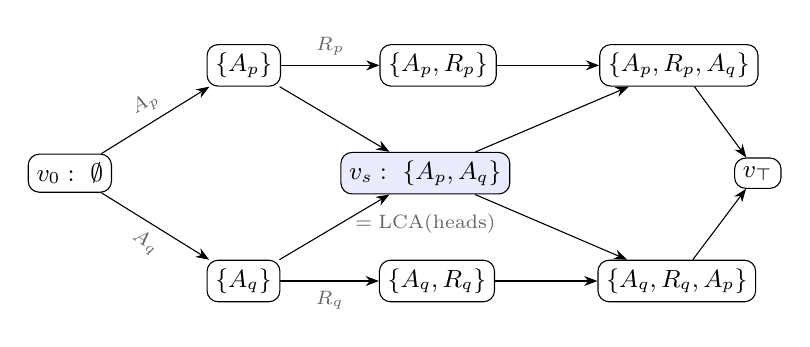
\begin{tikzpicture}[>=Stealth, node distance=0.55cm and 1.35cm,
  ver/.style={draw, rounded corners, inner sep=3pt, font=\small},
  lca/.style={draw, rounded corners, inner sep=3pt, font=\small,
    fill=blue!8},
  lbl/.style={font=\scriptsize, text=black!60}]
\node[ver] (v0) {$v_0:\ \emptyset$};
\node[ver, above right=0.85cm and 1.2cm of v0] (p1) {$\{A_p\}$};
\node[ver, below right=0.85cm and 1.2cm of v0] (q1) {$\{A_q\}$};
\node[lca, right=2.9cm of v0] (s) {$v_s:\ \{A_p,A_q\}$};
\node[ver, right=1.25cm of p1] (p2) {$\{A_p,R_p\}$};
\node[ver, right=1.25cm of q1] (q2) {$\{A_q,R_q\}$};
\node[ver, right=1.3cm of p2] (p3) {$\{A_p,R_p,A_q\}$};
\node[ver, right=1.3cm of q2] (q3) {$\{A_q,R_q,A_p\}$};
\node[ver, right=7.9cm of v0] (top) {$v_\top$};
\draw[->] (v0) -- node[lbl, above, sloped]{$A_p$} (p1);
\draw[->] (v0) -- node[lbl, below, sloped]{$A_q$} (q1);
\draw[->] (p1) -- (s);
\draw[->] (q1) -- (s);
\draw[->] (p1) -- node[lbl, above]{$R_p$} (p2);
\draw[->] (q1) -- node[lbl, below]{$R_q$} (q2);
\draw[->] (p2) -- (p3);
\draw[->] (s) -- (p3);
\draw[->] (q2) -- (q3);
\draw[->] (s) -- (q3);
\draw[->] (p3) -- (top);
\draw[->] (q3) -- (top);
\node[lbl, below=0.12cm of s] {$=\mathrm{LCA}(\text{heads})$};
\end{tikzpicture}
\caption{The ternary defeater (Example~\ref{ex:defeater}). Nodes are
versions labelled by their event sets; the shaded version $v_s$, created
by a staging replica, realizes $L(\text{head}_p)\cap L(\text{head}_q)$ as
an honest store version, so the final merge is LCA-legal. The removes
$R_p, R_q$ --- the only events a bottom-up derivation may peel last ---
are buried mid-history on their own sides.}
\label{fig:defeater}
\end{figure}

The consequences for the design are the same as binary, one level up: the
metatheorem must be rebuilt on canonical states and a Join Lemma, and its
merge-side VCs must be statements \emph{about the join}, not about how
either side's state factors.

\section{Canonical states and the ternary Join Lemma}
\label{sec:join}

The companion note's repair carries over verbatim on the update side ---
mechanically so: the replica-facing core of a ternary configuration
\emph{is} a binary configuration by projection, so the set-relative order
$\loE{E}$, its convergence theorem (any two $\loE{E}$-respecting
enumerations of $E$ fold to the same state), and hence \textbf{canonical
states} $\sigma(E)$ are literally reused, not re-proved. The one genuinely
ternary statement is what the merge must produce:

\begin{definition}[ternary Join Lemma]
For backward-closed event sets $E_1, E_2$ of a reachable configuration,
\[
  \sigma(E_1 \cup E_2)
  \;=\;
  \mergeL\bigl(\sigma(E_1 \cap E_2),\; \sigma(E_1),\; \sigma(E_2)\bigr).
\]
\end{definition}

By Lemma~\ref{lem:lca} the first argument is exactly the state the store
hands the merge. The adequacy proof (\S\ref{sec:adequacy}) is then an
induction over the transition system maintaining ``every version holds the
canonical state of its event set''; the merge case \emph{is} the Join
Lemma. What remains is the question this note exists to answer: which
per-data-type VCs make the Join Lemma true?

\section{Why the contract is a delta contract}
\label{sec:whydelta}

In the binary world the answer was lattice-flavoured: associativity,
idempotence and update-inflation, plus one contextual bound. Each of the
three provably fails to survive the lift.

\paragraph{No idempotence.} $\mergeL(l,a,a) = 2a - l$ for the counter:
only feasible \emph{triples} (where $l$ is the canonical state of the
intersection --- here, $l = a$) are idempotent. Unconditional idempotence
would exclude the counter, i.e.\ exclude precisely the data types the
ternary theorem exists for.

\paragraph{No usable order.} The binary route's workhorse order
$x \sqsubseteq y \coloneqq \Merge(x,y) = y$ has ternary candidates
$x \sqsubseteq_l y \coloneqq \mergeL(l,x,y) = y$, but for the counter this
relation degenerates to $x = l$; there is no antisymmetry left to split
proof obligations into a ``free half'' and a bounded half. The single
contextual VC below is accordingly an \emph{equation}, not an inequality.

\paragraph{Associativity is the wrong target.} The natural guess ---
$\mergeL(l,\mergeL(l,a,b),c) = \mergeL(l,a,\mergeL(l,b,c))$ --- assumes
one LCA for all three merges. In an execution, re-associating a three-way
reconciliation involves \emph{four} distinct LCAs:
\[
  \mergeL\bigl(l_{(ab)c},\, \mergeL(l_{ab}, a, b),\, c\bigr)
  \;\overset{?}{=}\;
  \mergeL\bigl(l_{a(bc)},\, a,\, \mergeL(l_{bc}, b, c)\bigr),
\]
with $l_{ab} = \sigma(E_a \cap E_b)$, $l_{(ab)c} = \sigma((E_a \cup E_b)
\cap E_c)$, and so on. For the counter --- whose canonical states are
additive measures over event sets --- the two sides come to $a+b+c$ minus
the two LCA measures, and they agree because
\[
  (E_a \cup E_b) \cap E_c = (E_a \cap E_c) \cup (E_b \cap E_c)
  \quad\Longrightarrow\quad
  \text{both LCA-sums} = |E_{ab}| + |E_{ac}| + |E_{bc}| - |E_{abc}|
\]
by inclusion--exclusion. The law holds, but only \emph{through the
set-algebra of intersections}: over four unconstrained states it is false.
Honest associativity is inherently a feasible-tuple fact --- and, the
mechanization's pleasant surprise, \textbf{the corrected induction never
needs it}. Every merge the induction forms already sits at its honest LCA;
the only laws consumed are two \emph{redistribution} identities that
equate two honestly-formed merges:

\begin{definition}[the delta contract]
\label{def:delta}
\begin{align*}
\textsc{local-redistribute}:&\quad
  \mergeL(l,\, \mergeL(m, x, c),\, y) \;=\; \mergeL(m,\, \mergeL(l, x,
  y),\, c),\\
\textsc{redistribute}:&\quad
  \mergeL\bigl(\mergeL(m,x_0,c),\, \mergeL(m,x_1,c),\, \mergeL(m,x_2,c)\bigr)\\
  &\qquad\qquad\qquad\;=\; \mergeL\bigl(m,\, \mergeL(x_0,x_1,x_2),\, c\bigr).
\end{align*}
\end{definition}

Read $c$ as a \emph{delta relative to $m$} (in the induction, $c$ will be
``apply event $e$ to its causal past''). \textsc{local-redistribute} says
a delta application commutes past an enclosing merge through one branch
slot. \textsc{redistribute} says a delta carried by \emph{all three}
components extracts \emph{once} --- the LCA slot cancels the duplicates by
arithmetic. This is the delta contract's quiet coup: cancelling the
duplicated shared contribution is exactly the job idempotence performed in
the binary theory, now done without any idempotence --- which is why the
counter sails through ($\textsc{redistribute}$ for the counter is the
identity $\sum x_i + 3c - 3m - (x_0 + c - m) - \cdots$ collapsing on both
sides).

\paragraph{Where the contract holds unconditionally --- and where it
cannot.} The two laws hold \emph{on all states} exactly for the
group-like class (the counter) and the lattice-like, LCA-blind class
(grow-only structures). They are \emph{unconditionally false} for the
OR-set: take an element tag present in $c$ and $l$ but in neither branch
--- the two sides of \textsc{local-redistribute} then disagree about
whether the LCA's copy survives. But such a tuple can never arise: a tag
in a canonical LCA state is in \emph{both} branches unless removed, and a
removal is itself an event of the branch. The failing tuples are
\emph{infeasible}, and this is a theorem-grade phenomenon, not an
inconvenience:

\begin{finding}
For LCA-sensitive MRDTs beyond the group $\oplus$ lattice classes, the
merge-coherence laws are irreducibly \emph{feasibility-conditioned}: true
on canonical tuples at honest LCAs, false in general. Quantifying merge
VCs over all states --- the published catalogue's style --- is not merely
inconvenient for such data types; for several laws it is wrong in
principle. (The enable-wins flag even falsifies the \emph{unit} law
$\mergeL(\Sinit,\Sinit,s)=s$ on an infeasible state with a set flag and a
zero counter.)
\end{finding}

Accordingly the delta laws enter the final contract in
feasibility-conditioned form: quantified over canonical states of
backward-closed event sets, with every $\mergeL$ node at its honest LCA.
The unconditional form remains available as a one-line \emph{on-ramp} (it
trivially implies the conditioned form) for the group and lattice
classes.

\section{The eight verification conditions}
\label{sec:vcs}

\begin{figure}[t]
\centering
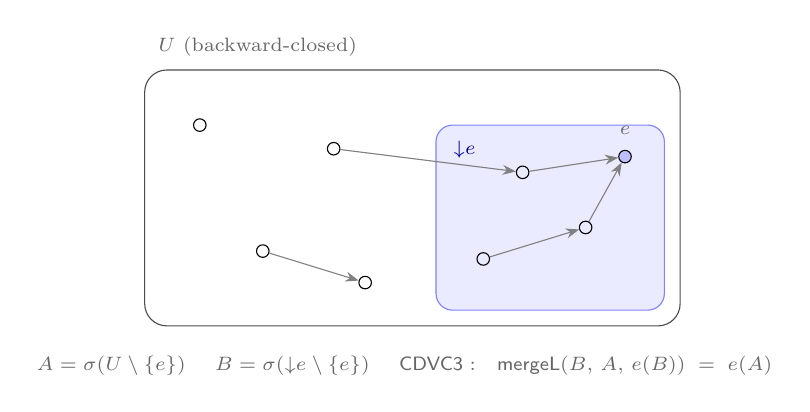
\begin{tikzpicture}[>=Stealth,
  ev/.style={circle, draw, inner sep=1.6pt, font=\scriptsize},
  lbl/.style={font=\scriptsize, text=black!60}]
% the big set U
\draw[rounded corners=8pt, black!70]
  (-0.4,-0.35) rectangle (6.4,2.9);
\node[lbl, anchor=south west] at (-0.35,2.95) {$U$ (backward-closed)};
% downset region
\begin{scope}[on background layer]
\fill[blue!8, rounded corners=6pt] (3.3,-0.15) rectangle (6.2,2.2);
\end{scope}
\draw[rounded corners=6pt, blue!50] (3.3,-0.15) rectangle (6.2,2.2);
\node[lbl, text=blue!60!black, anchor=north west] at (3.4,2.12) {$\dow{e}$};
% events
\node[ev] (x1) at (0.3,2.2) {};
\node[ev] (x2) at (1.1,0.6) {};
\node[ev] (x3) at (2.0,1.9) {};
\node[ev] (x4) at (2.4,0.2) {};
\node[ev] (y1) at (3.9,0.5) {};
\node[ev] (y2) at (4.4,1.6) {};
\node[ev] (y3) at (5.2,0.9) {};
\node[ev, fill=blue!25] (e) at (5.7,1.8) {};
\node[lbl, above=0.07cm of e] {$e$};
\draw[->, black!50] (y1) -- (y3);
\draw[->, black!50] (y2) -- (e);
\draw[->, black!50] (y3) -- (e);
\draw[->, black!50] (x3) -- (y2);
\draw[->, black!50] (x2) -- (x4);
\node[lbl] at (2.9,-0.85)
  {$A = \sigma(U\setminus\{e\})$ \quad
   $B = \sigma(\dow{e}\setminus\{e\})$ \quad
   $\cd:\ \ \mergeL(B,\, A,\, e(B)) \;=\; e(A)$};
\end{tikzpicture}
\caption{The causal-delta equation. The shaded region is $e$'s causal
past $\dow{e}$ (what $e$ saw); $e$ is $\loE{U}$-maximal. $e$'s effect on
the whole world $A$ equals: compute $e$'s effect on its own causal past
$B$, then merge that delta into $A$ \emph{over LCA $B$}. The merge sits at
its honest LCA: $(U\setminus\{e\}) \cap \dow{e} =
\dow{e}\setminus\{e\}$. Concurrent context that $e$ never observed
cannot amplify what $e$ does.}
\label{fig:cd}
\end{figure}

For an MRDT $\langle \Sigma, \Sinit, \mathsf{do}, \mergeL,
\mathsf{rc}\rangle$, the contract is:

\paragraph{Update layer (unconditional, SMT-shaped).}
\begin{enumerate}[leftmargin=2.2em]
\item \textbf{rc-non-comm (guarded)} --- for distinct events \emph{from
  different replicas}: they fail to commute iff $\mathsf{rc}$ orders them
  in exactly one direction. \emph{The conflict table is the commutativity
  table, with a direction.} The different-replica guard matters: it is
  the F\textsuperscript{*} artifact's own interface form
  (\lean{App\_mrdt.fsti}: \texttt{requires distinct\_ops o1 o2 /\char`\\\
  get\_rid o1 <> get\_rid o2}), dropped in an earlier transcription ---
  and the \emph{optimized OR-set} detects the drop: its same-replica
  same-element adds do not commute (the newer add evicts the older tag)
  yet are never concurrent, so $\mathsf{rc}$ rightly ignores them.
  Same-replica pairs are ordered by program order, not by conflict
  resolution.
\item \textbf{no-rc-chain} --- conflict priorities do not chain: never
  $o_1 \rc o_2$ and $o_2 \rc o_3$. This is what makes the linearization
  order acyclic, so maximal events exist --- the entire peel-and-recurse
  architecture stands on it.
\item \textbf{cond-comm} --- a resolved conflict is invisible once an
  absorber runs: swapping an $\mathsf{rc}$-ordered concurrent pair deep in
  a fold changes nothing for any later non-commuting event, across
  arbitrary intervening events. This is the engine of convergence.
\end{enumerate}

\paragraph{Merge layer.}
\begin{enumerate}[leftmargin=2.2em]\setcounter{enumi}{3}
\item \textbf{merge symmetry} --- $\mergeL(l,a,b) = \mergeL(l,b,a)$.
\item \textbf{feasible unit} --- $\mergeL(\Sinit,\Sinit,\sigma(E)) =
  \sigma(E)$: merging over nothing is a no-op, on states that can arise.
\item \textbf{feasible local-redistribute} and
\item \textbf{feasible redistribute} --- Definition~\ref{def:delta},
  quantified over canonical tuples at honest LCAs.
\item \textbf{the causal-delta equation ($\cd$)} --- for a
  $\loE{U}$-maximal event $e$ of a backward-closed $U$, with
  $A = \sigma(U\setminus\{e\})$ and $B = \sigma(\dow{e}\setminus\{e\})$
  the canonical state of $e$'s own causal past:
  \[
    \mergeL\bigl(B,\; A,\; e(B)\bigr) \;=\; e(A).
  \]
  \emph{What an event does is determined by what it saw}
  (Figure~\ref{fig:cd}): applying $e$ to the whole world equals computing
  $e$'s delta on its causal past and merging it in over that past.
\end{enumerate}

Items 1--4 are one-liners for every data type we have discharged; items
6--7 frequently hold unconditionally anyway (for the OR-set,
\textsc{redistribute} is a pointwise Boolean tautology); essentially the
entire per-data-type proof effort concentrates in item 8, whose discharge
follows a uniform recipe: characterize $\sigma(E)$ (a ``sandwich''
invariant along canonical enumerations), then a \emph{trichotomy} placing
every event the maximal $e$ interacts with either inside $\dow{e}$ or
absorbed on a side that owns it.

Compare the published catalogue: 24~VCs per data type, plus five more the
soundness proof uses silently. Seventeen of the~24 --- the
\textsc{BottomUp} induction-scheme families --- exist to drive the broken
induction and are consumed nowhere in the corrected one; the paper's
\textsc{MergeIdempotence} is likewise never used. The seventeen were,
however, doing honest work of a different kind: they are an
\emph{automation layer}, Skolemizing ``holds on feasible states'' into
base-and-step equations an SMT solver can discharge. Rebuilding that
layer, aimed at the corrected target ($\cd$ rather than \textsc{BottomUp}),
is in our view the most valuable open engineering problem this work
leaves (\S\ref{sec:open}).

\section{Adequacy}
\label{sec:adequacy}

\begin{theorem}[soundness of the eight VCs]
\label{thm:main}
If an MRDT satisfies VCs 1--8, then every configuration reachable from
the initial configuration in the ternary transition system is
RA-linearizable, per version.
\hfill\lean{ra\_linearizable\_of\_core\_feasible\_cd3}
\end{theorem}

The proof shape: the update layer powers the set-relative convergence
theorem, hence canonical states; the transition induction maintains
``every store version is canonical for its event set'' (fork and query
are trivial; apply is the extend lemma); the merge case reduces, via
Lemma~\ref{lem:lca}, to the ternary Join Lemma, which is proved from VCs
4--8 by strong induction on $|E_1 \cup E_2|$: select a
$\loE{E_1\cup E_2}$-maximal $e$, decompose each side containing $e$
through $\dow{e}$ (\textsc{local-redistribute} at the honest LCA
$\dow{e}\setminus\{e\}$), cancel the shared delta
(\textsc{redistribute}), close the principal step with $\cd$, and recurse.
The buried-event pathology of Example~\ref{ex:defeater} dissolves
structurally: no step ever asks how a \emph{side's} state factors ---
every factoring happens through the join.

Everything else one might fear owing is proved once, for all data types,
as an execution-model invariant: visibility transitivity, per-version
backward closure, store well-formedness, and Lemma~\ref{lem:lca} itself.
The data type owes exactly the eight equations.

\paragraph{A second route, and an honest asymmetry.} One discharged data
type does not fit the pattern above. The enable-wins flag's merge
\emph{compares counters} against the LCA, and for such merges the Join
Lemma's hypotheses as stated (backward closure under
non-commuting-visibility) are provably too weak: there is a
closure-legal tuple --- a live LCA enable, a dead post-LCA enable
inflating one side's counter, the killing disable visible only to the
other side --- on which the production merge computes the wrong flag. Full
\emph{causal} closure (which the store invariant actually supplies)
excludes it, and the flag is discharged through a full-closure variant of
the join. The finding: \textbf{required closure strength is a function of
the merge's shape} --- commutation-closure suffices for set-shaped merges,
counter-comparison merges need full causal closure. Reunifying the two
routes under one contract (full closure only strengthens what a data type
may assume) is open and, we expect, routine.

\section{The catalogue, discharged}
\label{sec:catalog}

\begin{table}[t]
\centering
\footnotesize
\resizebox{\textwidth}{!}{%
\begin{tabular}{@{}llll@{}}
\toprule
MRDT & contract tier & end-to-end theorem & $\sigma$-characterization (one line) \\
\midrule
Grow-only set & unconditional & \lean{goset\_ra\_linearizable3} & union of adds \\
Grow-only map & unconditional & \lean{gomap\_ra\_linearizable3} & union of $(k,v)$ records \\
Incr.-only counter & unconditional & \lean{ioc\_ra\_linearizable3} & $\#$events \\
PN-counter & unconditional & \lean{pn\_ra\_linearizable3} & $\#\mathsf{inc}-\#\mathsf{dec}$ \\
RGA (tombstone) & unconditional & \lean{rga\_ra\_linearizable3} & grow-only nodes + tombstones \\
Peritext & unconditional & \lean{peritext\_ra\_linearizable3} & grow-only mark records \\
OR-set & feasible & \lean{ORSet\_ra\_linearizable3} & tag live iff added, no vis-later $\rem$ \\
OR-set (efficient) & feasible & \lean{ORSetE\_ra\_linearizable3} & \dots{} or same-replica $\add$ later (eviction) \\
Enable-wins flag & full-closure & \lean{EWFlag\_ra\_linearizable3} & per key: ctr $=\#$enables; flag iff unkilled enable \\
\midrule
Multi-valued register & feasible & \multicolumn{2}{l}{recipe (trichotomy-free: all-comm $\Rightarrow B{=}\Sinit$)} \\
Add-wins priority queue & feasible & \multicolumn{2}{l}{recipe (the OR-set pattern on the add component)} \\
RGA (tombstone-free) & \emph{blocked} & \multicolumn{2}{l}{feasible \emph{update} layer needed (below)} \\
\bottomrule
\end{tabular}}
\caption{The Sal production catalogue against the eight VCs. Nine of
twelve carry kernel-checked end-to-end RA-linearizability; all discharges
live in a single \lean{MRDT\_Instances.lean}.}
\label{tab:catalog}
\end{table}

Table~\ref{tab:catalog} is the empirical heart of the note: the VC set is
not merely adequate in principle --- the data types people actually ship
satisfy it. Three lessons from the sweep:

\paragraph{Tombstones are a metatheoretic trivializer.} The catalogue's
celebrated hard cases --- the RGA sequence type and the Peritext
rich-text type --- land in the \emph{easiest} tier. The reason is almost
embarrassing: with tombstones, deletion \emph{adds} a record; every state
component is grow-only; all operations commute; the merge is a blind
join. All of the RGA's genuine difficulty lives in the \emph{read-side}
traversal (turning the node soup into a sequence), which
RA-linearizability of the state never touches. By contrast the
\emph{tombstone-free} RGA --- which physically deletes and repairs
positions by climbing ancestor paths --- is the one data type the theory
cannot yet host, for a reason worth stating precisely: its commutation VC
is itself \emph{reachability-conditioned} (two inserts commute only on
well-formed states), and our update layer, like the paper's, quantifies
over all states. The missing piece is a feasible \emph{update} layer ---
update VCs conditioned on an update-and-merge-closed invariant, plus a
transport lemma showing every state a canonical enumeration folds through
satisfies it. That is the theory's sharpest open edge, and precisely the
question the tombstone-free RGA was built to force.

\paragraph{Commutation class and delta class are independent axes.} The
multi-valued register is all-commuting, yet \emph{not} in the
unconditional tier: its merge is intersection-shaped,
$(l \cap a \cap b) \cup (a \setminus l) \cup (b \setminus l)$, and fails
the delta laws on infeasible tuples exactly as the OR-set does. The
boundary between tiers is drawn by \emph{how the merge uses its LCA}, not
by whether operations commute. (The compensation: all-commuting makes
every punctured causal past empty, $B = \Sinit$, so the feasible
discharge needs no trichotomy at all.)

\paragraph{The eight VCs certify real code on its historical fault
line.} The enable-wins flag's repository history contains a
known-broken sibling: a global-counter variant whose compositional VC
(\lean{inter\_right\_1op}) fails on DAG-shaped executions, the very defect
per-replica counters were introduced to fix. The mechanized $\sigma$-facts
prove the production merge computes exactly union-liveness ---
\emph{verified on precisely the corner where the sibling fails}. This is
the methodology working as intended: the metatheory does not merely bless
the catalogue, it explains \emph{why} the fixed design is right.

\section{Open questions}
\label{sec:open}

\begin{openq}[$\cd$-derivability]
Is $\cd$ derivable from VCs 1--7 (plus the unconditional delta laws where
they hold)? The binary analogue is pinned exactly --- there, the
corresponding causal-delta bound is \emph{equivalent} to the Join Lemma
and no strictly weaker bridge VC exists --- with both attack routes
characterized: the positive induction is circular at two identified case
shapes, and the countermodel space is narrowed to non-atomic lattice
states.
\end{openq}

\begin{openq}[structure theorem]
Empirically, the \emph{unconditional} delta contract holds exactly on the
group and lattice classes. Is every unconditional-$\mathsf{DeltaVCs3}$
merge a torsor-like group$\,\otimes\,$lattice combination? (The na\"ive
two-sorted umbrella $\mergeL(l,a,b) = a \boxplus (b \boxminus l)$ does
\emph{not} derive the contract uniformly, so the question is genuinely
open.)
\end{openq}

\begin{openq}[route reunification]
State the delta laws and $\cd$ over \emph{full causal closure} so the
enable-wins flag's route becomes an instance of the general one. Full
closure only strengthens the discharger's hypotheses; all current
discharges should port unchanged.
\end{openq}

\begin{openq}[the feasible update layer]
Condition the update-layer VCs on an update-and-merge-closed invariant
(with the permutation-transport lemma along canonical enumerations), and
host the tombstone-free RGA. The required invariant machinery
($\mathsf{RgaInv} \wedge \mathsf{id\_mono}$, closed under merge given
id-monotone allocation) is already mechanized on the data-type side.
\end{openq}

\begin{openq}[the automation layer]
The published catalogue's seventeen induction-scheme VCs were an
SMT-facing Skolemization of feasibility, aimed at the wrong target.
Design the analogous per-data-type induction scheme whose induction
implies $\cd$ and the feasible delta laws --- restoring push-button
discharge, now of VCs that actually imply RA-linearizability. The
observed uniformity of the discharges ($\sigma$-characterization by
sandwich invariant + absorber trichotomy) suggests the scheme exists.
\end{openq}

\section{Mechanization}
\label{sec:mech}

Everything above is mechanized in Lean~4 (Mathlib; axioms:
\lean{propext}, \lean{Classical.choice}, \lean{Quot.sound}; no
\lean{sorryAx} anywhere) in the Sal repository, under
\lean{Sal/MRDTs/Metatheory/}:

\begin{center}
\footnotesize
\resizebox{0.95\textwidth}{!}{%
\begin{tabular}{@{}lll@{}}
\toprule
Artifact & Lean & File \\
\midrule
signature, ternary $\mathsf{lo}$ & \lean{MRDTSig}, \lean{ConditionedMRDTSig} & \lean{MRDTSig.lean} \\
store, DAG, transitions & \lean{Configuration}, \lean{Step3} & \lean{ExecutionModel.lean}, \lean{LCA\_Lemma.lean} \\
Lemma~\ref{lem:lca} & \lean{lca\_events\_of\_storeInv} & \lean{LCA\_Lemma.lean} \\
$\sigma$/$\loE{E}$ layer (reused binary) & \lean{UpdateVCs}, \lean{IsCanonicalState} & \lean{Sigma\_LoOn3.lean} \\
the eight VCs & $\co$, $\fd$, $\cd$ & \lean{VC\_Set.lean} \\
Theorem~\ref{thm:main} + bridges & \lean{ra\_linearizable\_of\_core\_}\lean{feasible\_cd3} & \lean{Adequacy.lean} \\
Table~\ref{tab:catalog} & all instance theorems & \lean{MRDT\_Instances.lean} \\
Theorem~\ref{thm:counter-sep}, kill-tests & --- & \lean{Development/Impossibility.lean} \\
findings journal T0--T11 & --- & \lean{Development/MRDT\_METATHEORY\_DRAFT.md} \\
\bottomrule
\end{tabular}}
\end{center}

The binary theory this builds on --- including the refutations of the
original route, the CD ladder, and the exactness of the causal-delta
bound --- lives in \lean{Sal/CRDTs/Metatheory/} and is the subject of the
companion note. The production data types of Table~\ref{tab:catalog} are
mirrored faithfully from \lean{Sal/MRDTs/}$\ast$ (encoding deviations
documented per instance); their original 24-VC discharges are untouched.

\end{document}
